\documentclass[../../Main.tex]{subfiles}

\begin{document}
    \begin{figure}[hbt!]
        \centerline{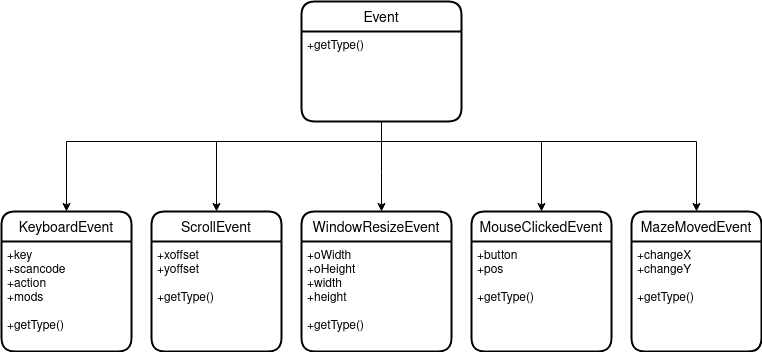
\includegraphics[scale=0.5]{img/Classes/Events.png}}
        \caption{Event subclasses}
        \label{fig}
    \end{figure}
    Event
    \begin{center}
        Functions
        \begin{tabular}{ | m{0.15\textwidth} | m{0.35\textwidth}| m{0.4\textwidth} | }
            \hline
            \textbf{Function Name} & \textbf{Parameters} & \textbf{Description} \\
            \hline
            getType & & Returns the type of event \\
            \hline
        \end{tabular}
    \end{center}
    keyboardEvent
    \begin{center}
        Variables
        \begin{tabular}{ | m{0.45\textwidth} | m{0.45\textwidth} | }
            \hline
            \textbf{Variable Name} & \textbf{Description} \\
            \hline
            key & Stores the key pressed \\
            \hline
            scancode & Stores the platform-specific scancode \\
            \hline
            action & Stores the action of the key (Release, press, hold)\\
            \hline
            mods & Stores the modifier bits \\
            \hline
        \end{tabular}
    \end{center}
    ScrollEvent
    \begin{center}
        Variables
        \begin{tabular}{ | m{0.45\textwidth} | m{0.45\textwidth} | }
            \hline
            \textbf{Variable Name} & \textbf{Description} \\
            \hline
            xoffset & Stores the change in the x direction \\
            \hline
            yoffset & Stores the change in the y direction \\
            \hline
        \end{tabular}
    \end{center}
    WindowResizeEvent
    \begin{center}
        Variables
        \begin{tabular}{ | m{0.45\textwidth} | m{0.45\textwidth} | }
            \hline
            \textbf{Variable Name} & \textbf{Description} \\
            \hline
            oWidth & Stores the width before the transformation \\
            \hline
            oHeight & Stores the height before the transformation \\
            \hline
            width & Stores the new width \\
            \hline
            height & Stores the new height \\
            \hline
        \end{tabular}
    \end{center}
    MouseClickedEvent
    \begin{center}
        Variables
        \begin{tabular}{ | m{0.45\textwidth} | m{0.45\textwidth} | }
            \hline
            \textbf{Variable Name} & \textbf{Description} \\
            \hline
            button & Stores the button that has been pressed \\
            \hline
            pos & Stores the position of the mouse \\
            \hline
        \end{tabular}
    \end{center}
    MazeMovedEvent
    \begin{center}
        Variables
        \begin{tabular}{ | m{0.45\textwidth} | m{0.45\textwidth} | }
            \hline
            \textbf{Variable Name} & \textbf{Description} \\
            \hline
            changeX & Stores the change in X that has happened \\
            \hline
            changeY & Stores the change in Y that has happened \\
            \hline
        \end{tabular}
    \end{center}
\end{document}